\chapter{Results}
\label{cha:results}
\section{Graphene on Ir(111)}

The quality of the graphene was checked before each dose of D$_2$, in order to ensure that the amount of defects was at a minimum. STM images of pure graphene on Ir(111) are shown in this section. On figure \ref{GrIr} images of graphene on Ir(111) in different sizes are shown. Figure \ref{GrIr1} shows a large image of a graphene monolayer covering the Ir(111) surface. Although the quality of the image is low, the moire pattern can be perceived as a pattern of small hexagonal structures, as outlined in the top left of the image. Also several step edges from the underlying Ir surface is seen. Several line scans has been performed on these edges, which show that the height difference is 2Å $\pm$0.4Å. This value is consistent with the value of 0.22nm found in the literature.\cite{1367-2630-11-2-023006}\\
On figure \ref{GrIr2} a high resolution image of Gr/Ir(111) is seen. The moire pattern is very prominent in this figure, which once again is outlined as the blue hexagon.  and the spacing between the individual sites in the moire unit cell can be determined from a line scan. A line scan was drawn on figure \ref{GrIr2} and two points were positioned in the corners of the moire unit cell in order to obtain the moire periodicity. The moiré periodicity is 25.2 $\pm$ 0.4Å according to the literature.\cite{1367-2630-10-4-043033} This agrees with the measured length of 25.24 $\pm$ 1 Å from the line scan, which is seen on figure \ref{linescan}. Typical defects of the graphene monolayer is seen as well in this figure, as seen within the blue circle. A close look at figure \ref{GrIr2} indicates that another periodic structure than the moiré pattern is present. This pattern is however more clear in figure \ref{GrIr3}. This image is a zoom in of the image shown in figure \ref{GrIr2} corresponding to the dashed square. The smaller pattern mentioned before is much more visible on this image. The hexagonal pattern is the graphene monolayer on top of the iridium. The graphene hexagon is sketched as the blue hexagon and the moiré pattern as seen on the two preceding figures is sketched as the dashed blue hexagon. The moiré unit cell is shown as well as the blue rhombus, where the four dark corners corresponds to the ATOP sites. The HCP and FCC sites lies at the corners of the dashed blue hexagon within the outlined moiré unit cell.

\begin{figure}[H]
\makebox[\textwidth][c]{
  \begin{subfigure}[b]{0.3\paperwidth}
    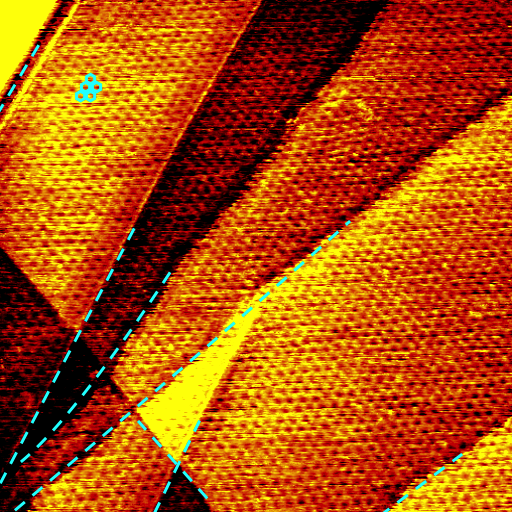
\includegraphics[height=\textwidth]{STMdata/FFT/2016-04-11_000_33.png}
    \caption{993x993 Å - 0.690 nA 78.1 mV}
    \label{GrIr1}
  \end{subfigure}
  \begin{subfigure}[b]{0.3\paperwidth}
    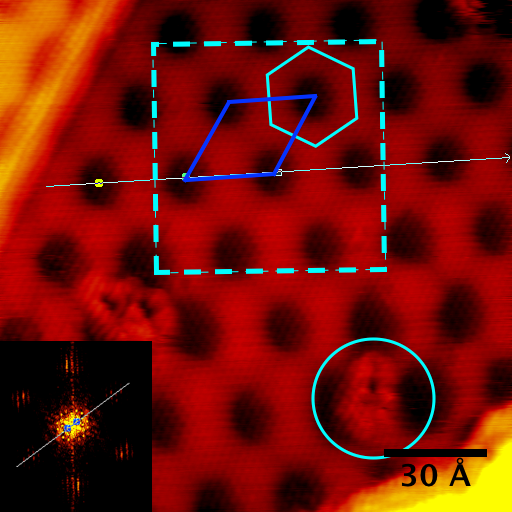
\includegraphics[height=\textwidth]{STMdata/FFT/2016-04-11_000_50.png}
    \caption{148x148 Å - -0.890 nA -311.3 mV}
    \label{GrIr2}
  \end{subfigure}
  \begin{subfigure}[b]{0.3\paperwidth}
    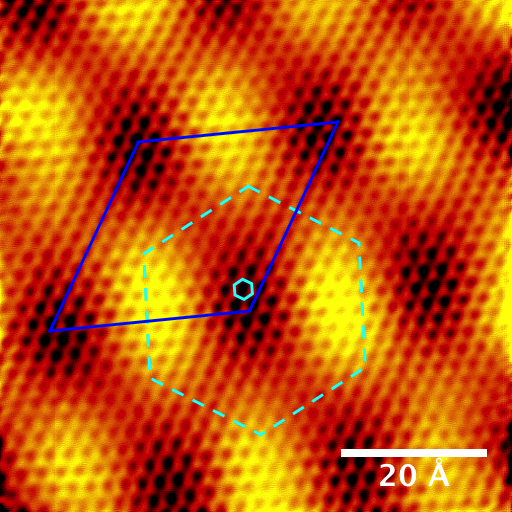
\includegraphics[height=\textwidth]{STMdata/FFT/2016-04-11_000_56.png}
    \caption{70x70 Å - 0.910 nA 311.3 mV}
    \label{GrIr3}
  \end{subfigure}
  }
  \\
\makebox[\textwidth][c]{
  \begin{subfigure}[b]{0.7\paperwidth}
    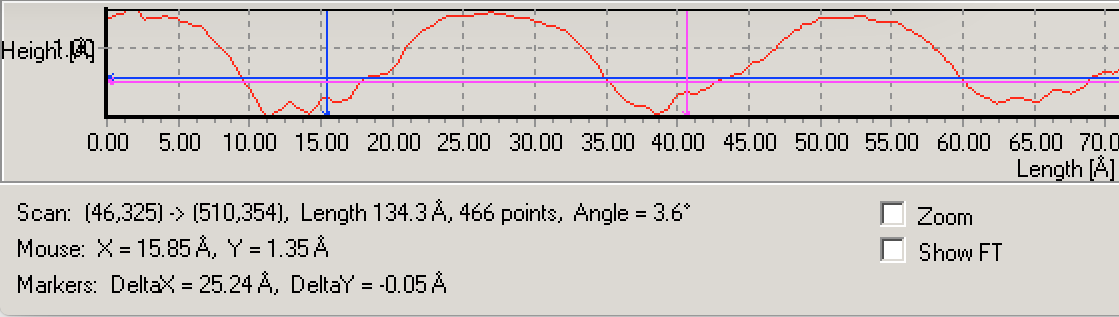
\includegraphics[width=\textwidth]{STMdata/FFT/Linescan}
    \caption{Line profile of the linescan in figure (b).}
    \label{linescan}
  \end{subfigure}
}
\caption{Clean graphene on Ir(111). (c) is a zoom in of (b) which is shown as the dashed square.}
\label{GrIr}
\end{figure}

\section{D$_2$ on graphene}

In the following sections, the data from the dose of vibrationally excited molecules are presented. It was desirable to determine the threshold temperature of the hydrogenation of graphene. Hence the temperature of the doser was varied in order alter the flux of atoms from the doser, and thereby changing the number of hydrogen recombinations on the walls within the chamber. Therefore the data includes dosages at temperatures of, 1343\degree C, 1543\degree C and 1745\degree C. A dose at 1300\degree C were performed as well, however the STM broke, and no pictures are therefore included.

\subsection{Full hydrogen coverage}
STM images were made from a fully hydrogenated surface in order to compare these to the images from the short dosages. The fully hydrogenated surface was made by filling the chamber with hydrogen at a pressure of $1 \cdot 10^{-5}$mbar and with the iongauge set to 1.0mA. These conditions were left for 12 hours and the sample was scanned afterwards. On figure \ref{D2:full} images on different scales can be seen. As seen on figure \ref{full:1} the sample is not just locally hydrogenated. Ring structures are seen covering the surface on this image, instead of the moiré pattern observed on figure \ref{GrIr1}. These structures are however more clear on the following figure \ref{full:2}, which is a zoom in of figure \ref{full:1}. The most common pattern, of the hydrogenated surface, is ring shaped as structures with a bright rim and a darker center. By comparing figure \ref{full:2} with figure \ref{GrIr2} it is obvious that the adsorption of hydrogen on the surface changes the LDOS. It is noticeable that the defects on figure \ref{GrIr2} looks like the ring shaped structures seen on figure \ref{D2:full}, and hence these defect might be caused by adsorbed hydrogen. Furthermore some H-structures on the saturated surface seem to melt together in a bigger structure, seen as the bone- and three point star shaped structures as pointed out in figure \ref{full:2}.
A line scan was performed on the sample in order to check the periodicity of the pattern on the hydrogenated surface. The line scan is seen on figure \ref{full:3} and the related profile is shown in figure \ref{linescan2}. The distance between the two points is measured to 24.2 $\pm$1 Å. This value is very close to the expected periodicity of the moiré unit cell.\cite{1367-2630-11-2-023006}\\

\begin{figure}[H]
\makebox[\textwidth][c]{
  \begin{subfigure}[b]{0.3\paperwidth}
    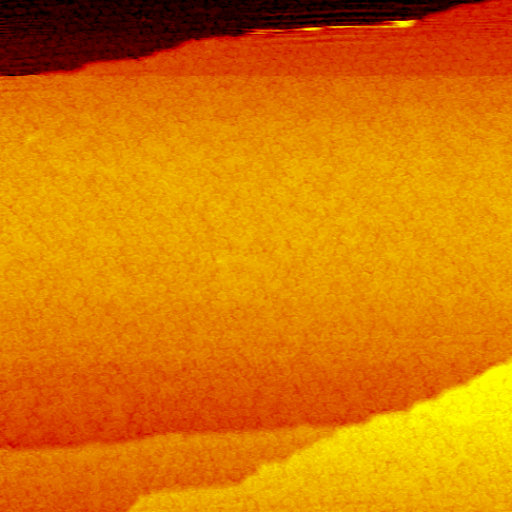
\includegraphics[height=\textwidth]{STMdata/FFT/2016-04-13_001_15.png}
    \caption{949x949 Å - 0.860 nA 67.1 mV}
    \label{full:1}
  \end{subfigure}
  \begin{subfigure}[b]{0.3\paperwidth}
    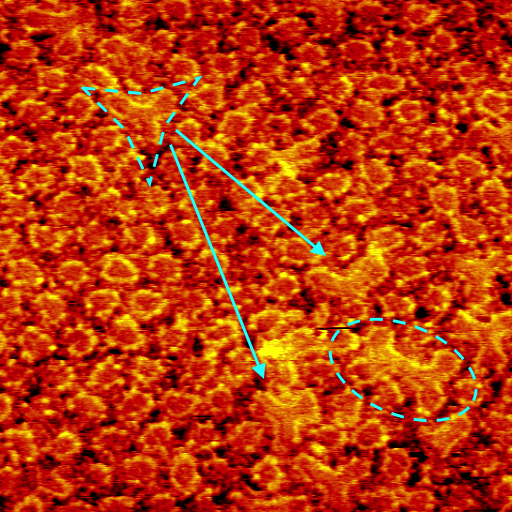
\includegraphics[height=\textwidth]{STMdata/FFT/2016-04-13_001_4.png}
    \caption{497x497 Å - 0.850 nA 73.5 mV}
    \label{full:2}
  \end{subfigure}
  \begin{subfigure}[b]{0.3\paperwidth}
    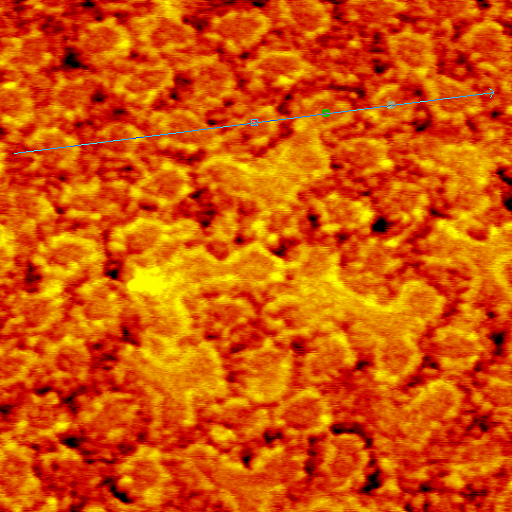
\includegraphics[height=\textwidth]{STMdata/FFT/2016-04-13_001_13.png}
    \caption{150x150 Å - 0.850 nA 73.5 mV}
    \label{full:3}
  \end{subfigure}
}
\\
\makebox[\textwidth][c]{
\begin{subfigure}[b]{0.7\paperwidth}
  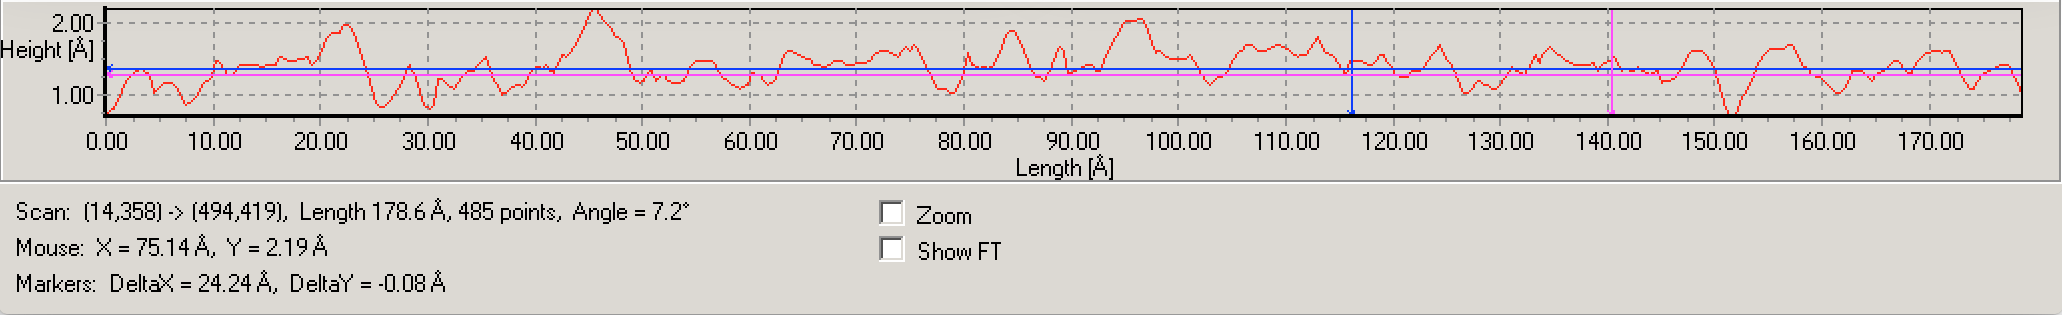
\includegraphics[width=\textwidth]{STMdata/FFT/LinescanfullH}
  \caption{Line profile of the linescan in figure (c).}
  \label{linescan2}
\end{subfigure}
}
\caption{Fully hydrogenated Gr/Ir(111) surface after 12h D$_2$ dosage. (c) is a zoom in on (b)}
\label{D2:full}
\end{figure}


\subsection{1745\degree C dose}

This dose was performed at a pirani pressure of $6.8 \cdot 10^{-2}$mbar, and with the doser at a temperature of 1745\degree C. The dosage time was 20 min. The graphene was checked before the dose in order to ensure that no abnormal amount of defects was present. Three images at different scales are shown in figure \ref{D2:1745}. These pictures were taken right after the dose had ended, and the pressure dropped sufficiently. As seen on figure \ref{D2:17451}, the surface is far from saturated, compared to figure \ref{full:1}, since the moiré pattern is seen in between areas where the distinct ring structure of the hydrogenation is seen. It is also worth noting that none of the hydrogenated sites melt together to form bigger structures, which indicates that this phenomenon happens as the surface becomes saturated.\\
In figure \ref{D2:1745} each moiré unit cell has been sketched out with blue dashed lines. From this it is obvious that hydrogenation only happens at one site in the bottom left corner of the moiré unit cell. Earlier studies suggest that this is the FCC site in the moiré unit cell.\cite{Jakobunpublished} It is, however, seen that the hydrogenation expands to the HCP site as well in some of the unit cells, as shown with the dark blue circle.\\
Individual hydrogen atoms are not distinguishable from the STM images, and therefore the coverage is estimated as a percentage of the number of hydrogenated unit cells to the total number of unit cells. Figures \ref{D2:17452} and \ref{D2:17453} were used to calculate an estimate of the hydrogenation of the surface. The coverage on figure \ref{D2:17452} was calculated to 41\% and the coverage on figure \ref{D2:17453} was calculated to 29\%. This means that about one third of the unit cells is hydrogenated after a dosage of excited molecules for 20 min, at a chamber pressure of $5 \cdot 10^{-5}$mbar.

\begin{figure}[H]
\makebox[\textwidth][c]{
  \begin{subfigure}[b]{0.3\paperwidth}
    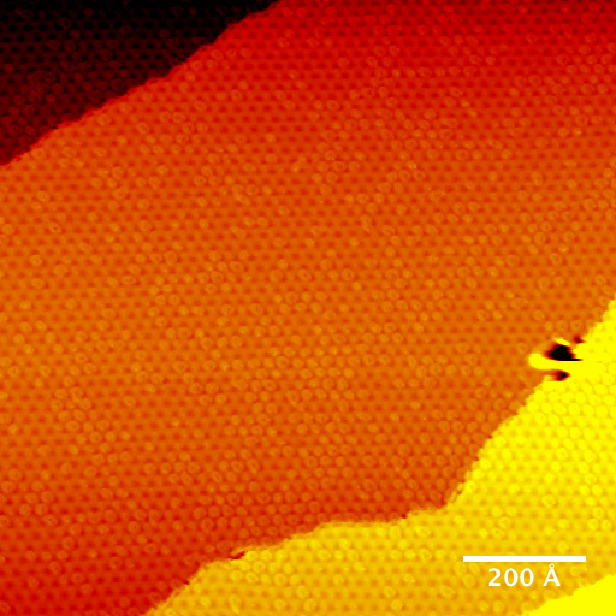
\includegraphics[height=\textwidth]{STMdata/FFT/2016-04-11_003_14.png}
    \caption{998x998 Å - 1.060 nA 67.1 mV}
    \label{D2:17451}
  \end{subfigure}
  \begin{subfigure}[b]{0.3\paperwidth}
    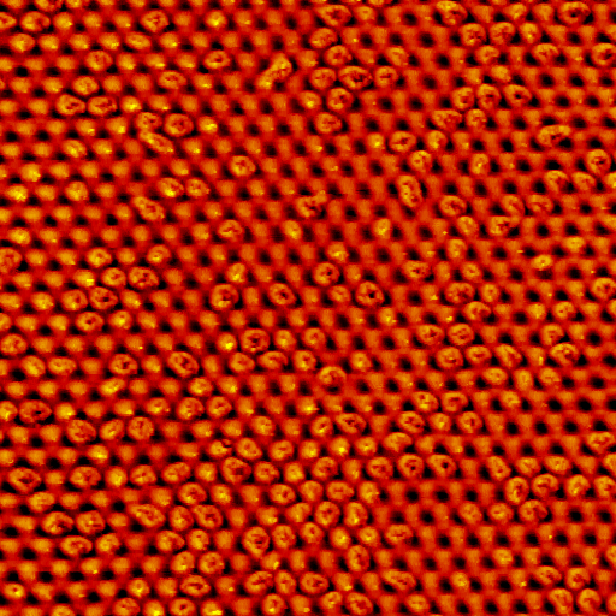
\includegraphics[height=\textwidth]{STMdata/FFT/2016-04-11_003_15.png}
    \caption{497x497 Å - 1.080 nA 67.1 mV}
    \label{D2:17452}
  \end{subfigure}
  \begin{subfigure}[b]{0.3\paperwidth}
    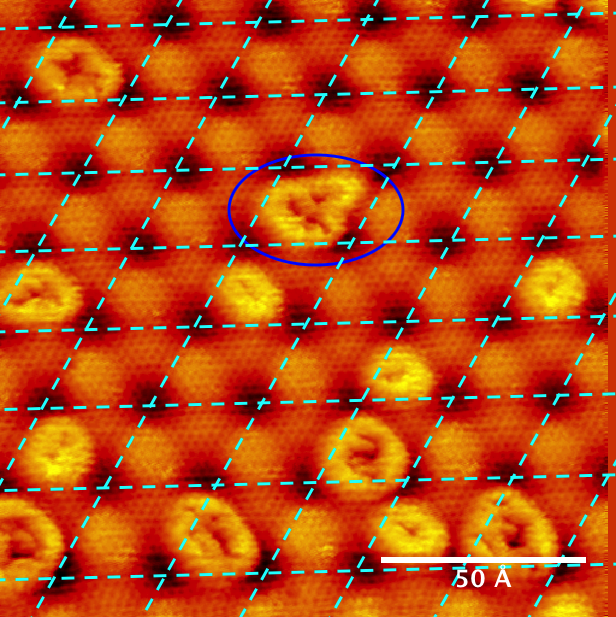
\includegraphics[height=\textwidth]{STMdata/FFT/2016-04-11_003_23.png}
    \caption{150x150 Å - 1.090 nA 67.1 mV}
    \label{D2:17453}
  \end{subfigure}
}
\caption{Hydrogenated Gr/Ir surface after dose of D$_2$ at a doser temperature of 1745\degree C.}
\label{D2:1745}
\end{figure}

\subsection{1593\degree C dose}

This dose was performed at a pirani pressure of $6.8 \cdot 10^{-2}$mbar and a doser temperature of 1593\degree C. Again the dose had a duration of 20 min. The images obtained after the dose are shown in figure \ref{D2:1593}. The resemblance between the pictures shown in figure \ref{D2:1745} and \ref{D2:1593} is quite high. Again the ring shaped structures are seen, and the shape of these are very similar to the ones observed earlier. Figures \ref{D2:15931} and \ref{D2:15932} were used to calculate the coverage of hydrogenation, with values of 32\% and 25\% respectively. These values are however very position dependant, and therefore they do not necessarily reflect the accurate coverage. It is however clear that hydrogenation of the surface has occurred.

\begin{figure}[H]
\makebox[\textwidth][c]{
  \begin{subfigure}[b]{0.3\paperwidth}
    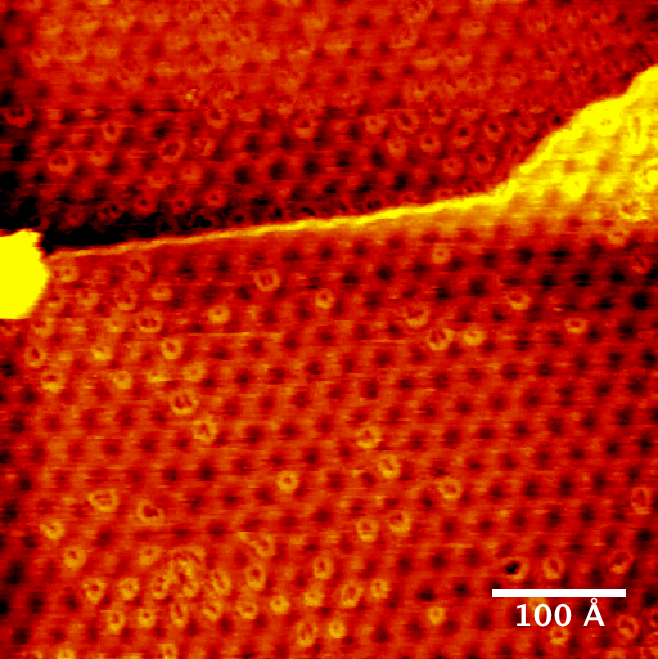
\includegraphics[height=\textwidth]{STMdata/FFT/2016-04-14_000_44.png}
    \caption{488x488 Å - 0.900 nA 190.4 mV}
    \label{D2:15931}
  \end{subfigure}
  \begin{subfigure}[b]{0.3\paperwidth}
    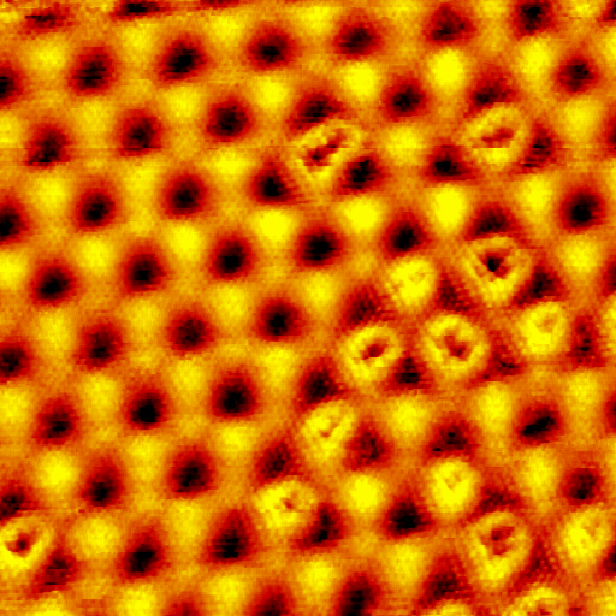
\includegraphics[height=\textwidth]{STMdata/FFT/2016-04-14_000_27.png}
    \caption{180x180Å - 1.020 nA 190.4 mV}
    \label{D2:15932}
  \end{subfigure}
  \begin{subfigure}[b]{0.3\paperwidth}
    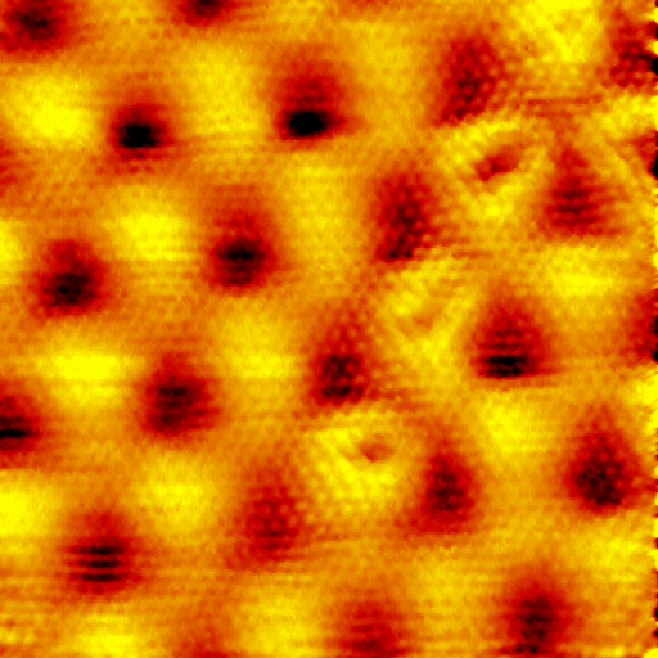
\includegraphics[height=\textwidth]{STMdata/FFT/2016-04-14_000_29.png}
    \caption{97x97 Å - 1.020 nA, 190.4 mV}
    \label{D2:15933}
  \end{subfigure}
}
\caption{Hydrogenated Gr/Ir surface after dose of D$_2$ at a doser temperature of 1593\degree C.}
\label{D2:1593}
\end{figure}

\subsection{1343\degree C dose}

The pirani pressure was measured to $6.8 \cdot 10^{-2}$mbar, and the doser had a temperature of 1343\degree C during this dose. Hydrogen was dosed for 20 min as earlier. As seen on figure \ref{D2:1340} several high quality pictures of the sample was taken. On figure \ref{D2:13401} it would seem like some hydrogen is adsorbed due to the observation of several ring shaped structures. As a smaller image is taken such as the one in figure \ref{D2:13402} the defects looks somewhat different from those seen earlier on figures \ref{D2:15932} and \ref{D2:17453}. The ring shaped structures are much smaller in diameter on figure \ref{D2:13402}, even though the scanning parameters are close to each other.\\
A high resolution image is seen on figure \ref{D2:13403}, where the hexagonal graphene is highly visible. On this picture it is clear that the graphene is defected, although it is unclear whether this is due to the presence of hydrogen. It is also seen that the shape of the sites in the moiré unit cell looks different than earlier although both pictures are from the same scan session. This is due to a tip effect, where the LDOS of the tip probably has changed, which has an influence on the tunnelling current. This  might happen if the tip picks up an atom from the surface, or if the physical dimensions of the tip changes after a tip treatment.\\
It should be noted that the graphene had defects before the dose was initiated. The abundance of these defects was indistinguishable, when comparing before and after the dose. Therefore it is not possible to conclude whether the threshold temperature of the hydrogen adsorption from excited molecules lies at 1340\degree C. It is however very likely that no hydrogen is adsorbed. In order to investigate the threshold temperature further, it would be rational to conduct TPD measurements of the sample after hydrogen dosage at 1343 \degree C.

\begin{figure}[H]
\makebox[\textwidth][c]{
  \begin{subfigure}[b]{0.3\paperwidth}
    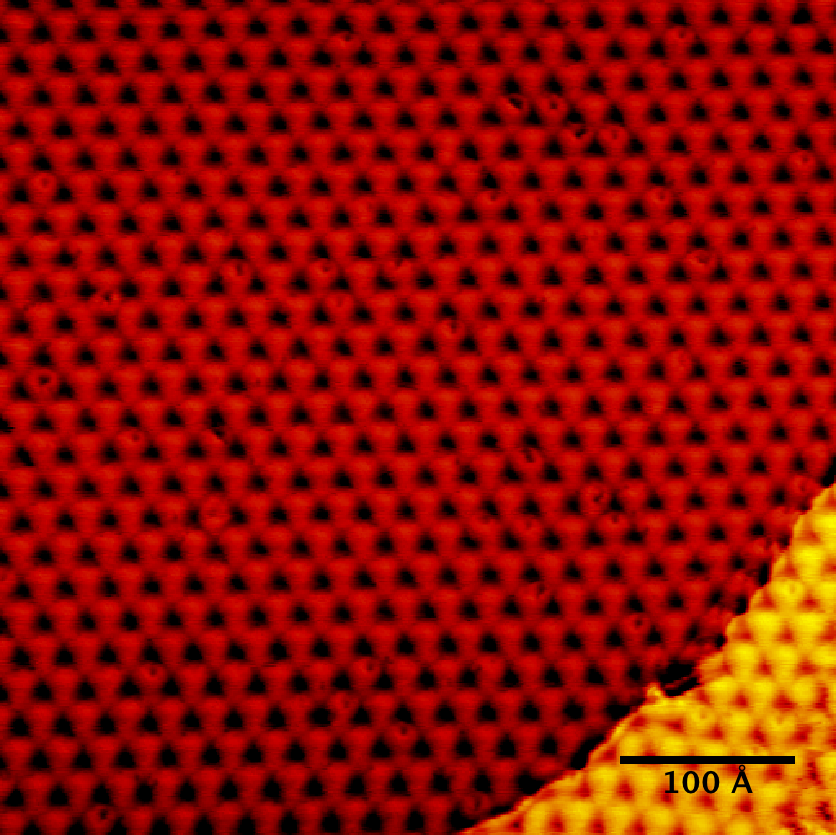
\includegraphics[height=\textwidth]{STMdata/FFT/2016-04-16_001_50_26.png}
    \caption{477x477 Å - 0.820 nA 20.1 mV}
    \label{D2:13401}
  \end{subfigure}
  \begin{subfigure}[b]{0.3\paperwidth}
    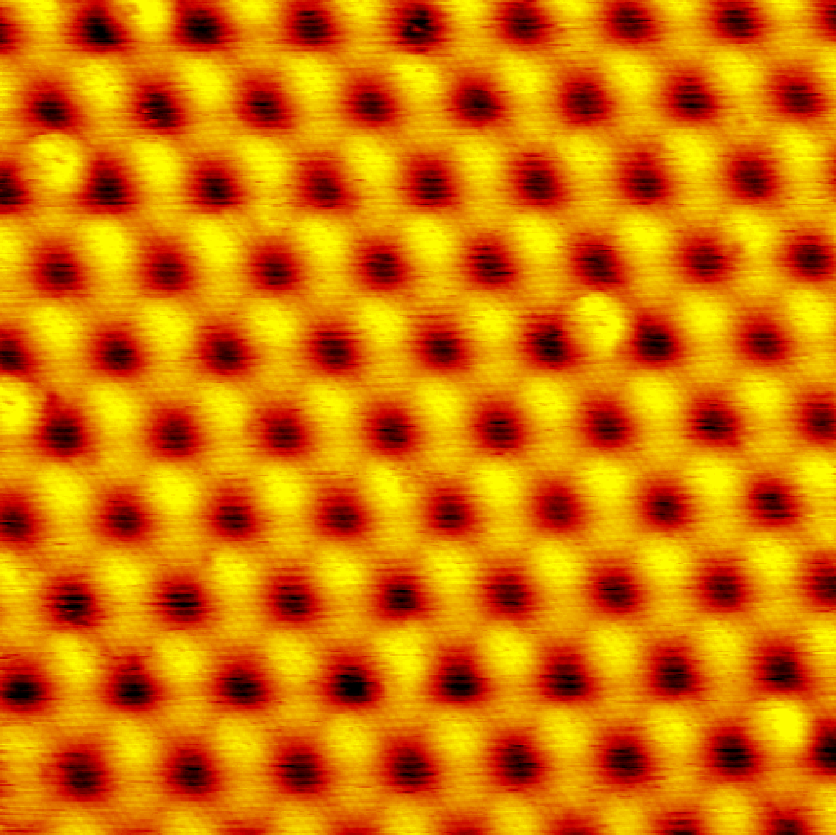
\includegraphics[height=\textwidth]{STMdata/FFT/2016-04-16_001_50_8.png}
    \caption{192x192Å - 0.830 nA 55.8 mV}
    \label{D2:13402}
  \end{subfigure}
  \begin{subfigure}[b]{0.3\paperwidth}
    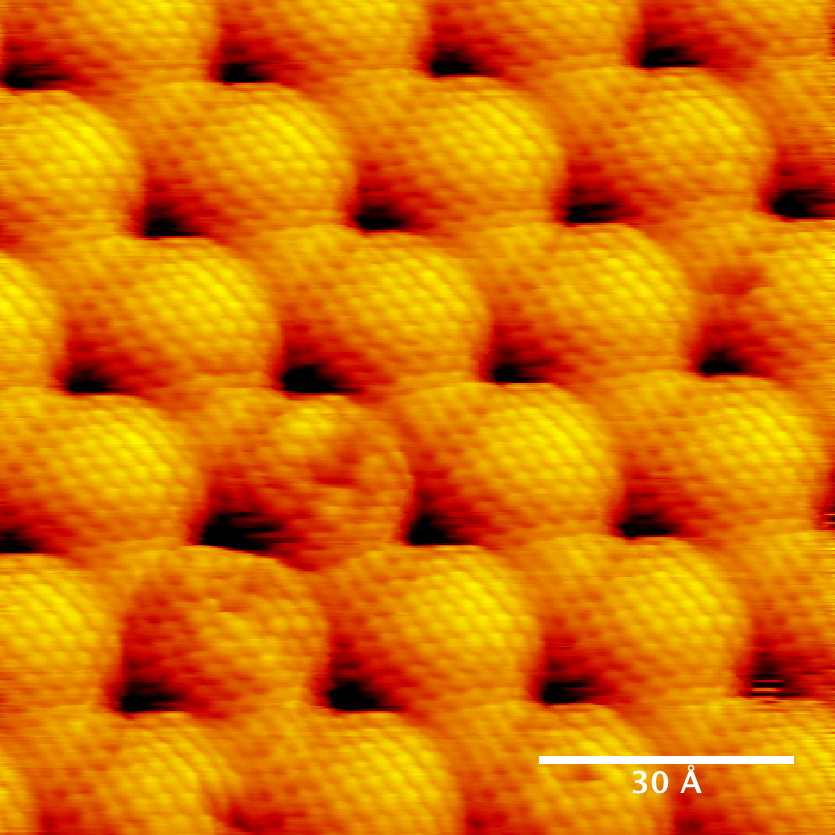
\includegraphics[height=\textwidth]{STMdata/FFT/2016-04-16_001_50_15.png}
    \caption{98x98 Å - 0.820 nA, 20.1 mV}
    \label{D2:13403}
  \end{subfigure}
}
\caption{Hydrogenated Gr/Ir surface after dose of D$_2$ at a doser temperature of 1340\degree C.}
\label{D2:1340}
\end{figure}


\section{TPD measurements}
In the following sections, TPD measurements from graphene on Ir(111) exposed to both hot molecules and atoms are compared. These data were gathered twice from two different samples as explained in chapter \ref{cha:procedure}. Furthermore the effect of a bilayered sample on the hydrogenation of graphene was investigated by conducting TPD measurements.

\subsection{Atomic and molecular D2}

In figure \ref{TPD:all} below, the data from the TPD is gathered in two different figures. TPD measurements were made following doses of both vibrationally excited molecules and atoms. Figure \ref{TPD:D2} shows the TPD data following a 60 min dose of D$_2$ at a chamber pressure of $5\cdot 10^{-7}$mbar and a doser temperature of 1740\degree C. Figure \ref{TPD:D} shows the data following a 60 min dose of hydrogen atoms at a chamber pressure of $5\cdot 10^{-7}$mbar and a doser temperature of 1740\degree C.\\
After dosage of excited molecules a single peak is observed. On figure \ref{TPD:D2} this peak is seen from two datasets matching the two different samples. It is worth noting that the peaks are shifted compared to each other. The reason for this might be the fact that the sample temperature was measured using two different thermocouples as explained in chapter \ref{cha:procedure}.For the second dataset, corresponding to the blue graph, a quite big peak is seen after the main peak, at a temperature of about 800K. This is due to a temperature spike caused by the Eurotherm temperature controller. The calibration of the Eurotherm during this experiment was poor, which results in noticeable fluctuations in the desorption of hydrogen. This phenomenon is also observed on figure \ref{TPD:D}, on the blue graph. This dataset was gathered during the same chamber and sample conditions as the blue graph in figure \ref{TPD:D2}. Therefore the calibration of the Eurotherm was poor as well, which is seen after the small peak at about 500K in figure \ref{TPD:D}. Here several small bumps are seen due to the non-linear temperature ramp.\\
The temperature at the peak was found by the procedure described in chapter \ref{cha:procedure}. The single peak in figure \ref{TPD:D2} must correspond to the hydrogen adsorbed on the HCP and FCC sites in the moiré unit cell. This statement is supported by the preceding STM pictures that show no sign of hydrogen dimers in the ATOP sites. The temperature of this peak was found for 6 datasets in all, and the values of these are shown in the table below, along with the mean value.\\
\begin{table}
  \centering
  \makebox[\textwidth][c]{
  \begin{tabular}{c|c|c|c|c|c|c|c}
    Sample & fig.\ref{TPD:D2} blue & fig.\ref{TPD:D2} green & fig.\ref{TPD:D} blue & fig.\ref{TPD:D} green & fig.\ref{TPD:bilayer} green & fig.\ref{TPD:bilayer} red & mean \\
    \hline
    Peak T [K] & 724.8 & 698.4 & 694.0 & 709.1 & 739.1 & 753.4 & 719.8
    %Peak E [meV] & 62.5 & 60.2 & 59.8 & 61.1 & 63.7 & 64.9 & 62.0
  \end{tabular}}
\end{table}
Another peak appears when observing the Gr/Ir sample after it has been dosed with hot atoms as seen on figure \ref{TPD:D}. The green graph was initially observed, and from this it is obvious that more hydrogen desorbs from the surface at lower temperature, compared to the green graph on figure \ref{TPD:D2}. After a second try however, an actual peak was observed. The temperature of this peak was found by the same procedures as earlier, and the value was found to be 550.4K. This suggests that a different type of Gr-H bond is present. The most plausible explanation is the presence of hydrogen dimers on the ATOP site of the moiré unit cell. The fact that no hydrogen adsorbs as dimers, when excited molecules are dosed, is supported heavily by the fact that this peak around 550K is completely absent from all the data obtained from the molecular dosage seen in figures \ref{TPD:D2} and \ref{TPD:bilayer}.

\begin{figure}
  \centering
  \begin{subfigure}[b]{0.45\textwidth}
    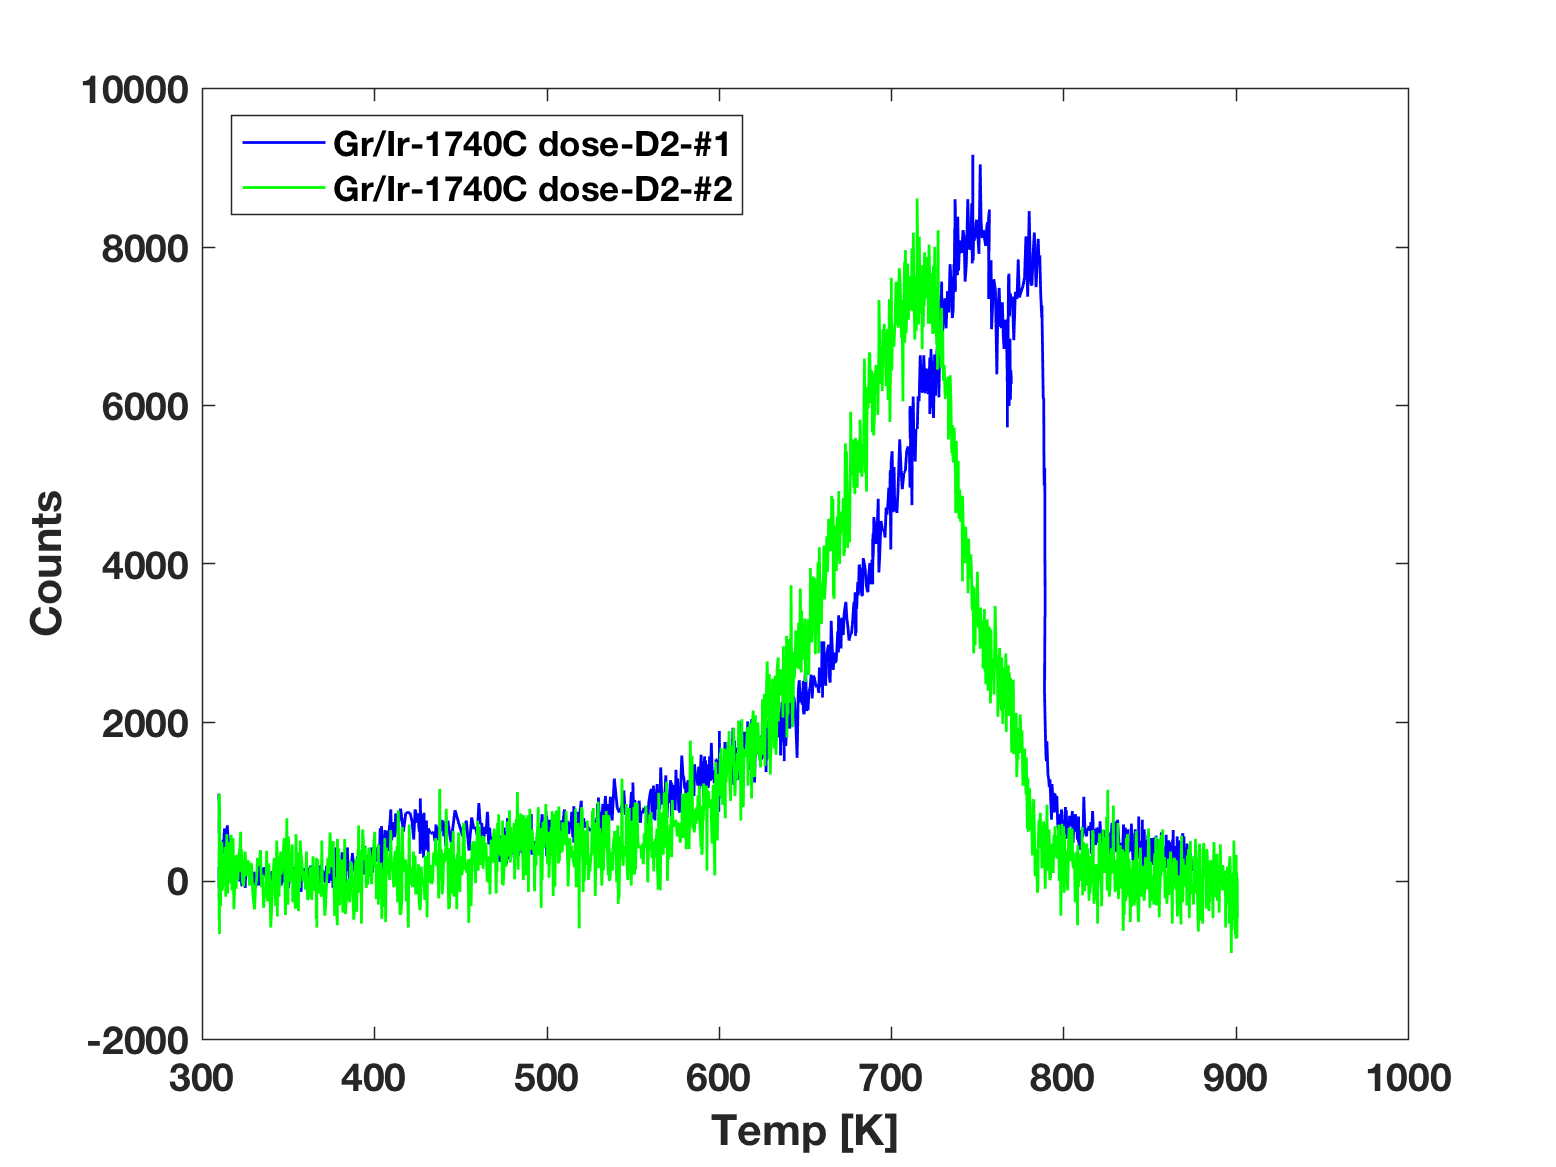
\includegraphics[width=\textwidth]{TPD/050516IrSorenD2dose1hourtemp.png}
    \caption{TPD of Gr/Ir after 1 hour dose of D$_2$ with a doser temperature of 1740 \degree C.}
    \label{TPD:D2}
  \end{subfigure}\hspace{0.5cm}
  \begin{subfigure}[b]{0.45\textwidth}
    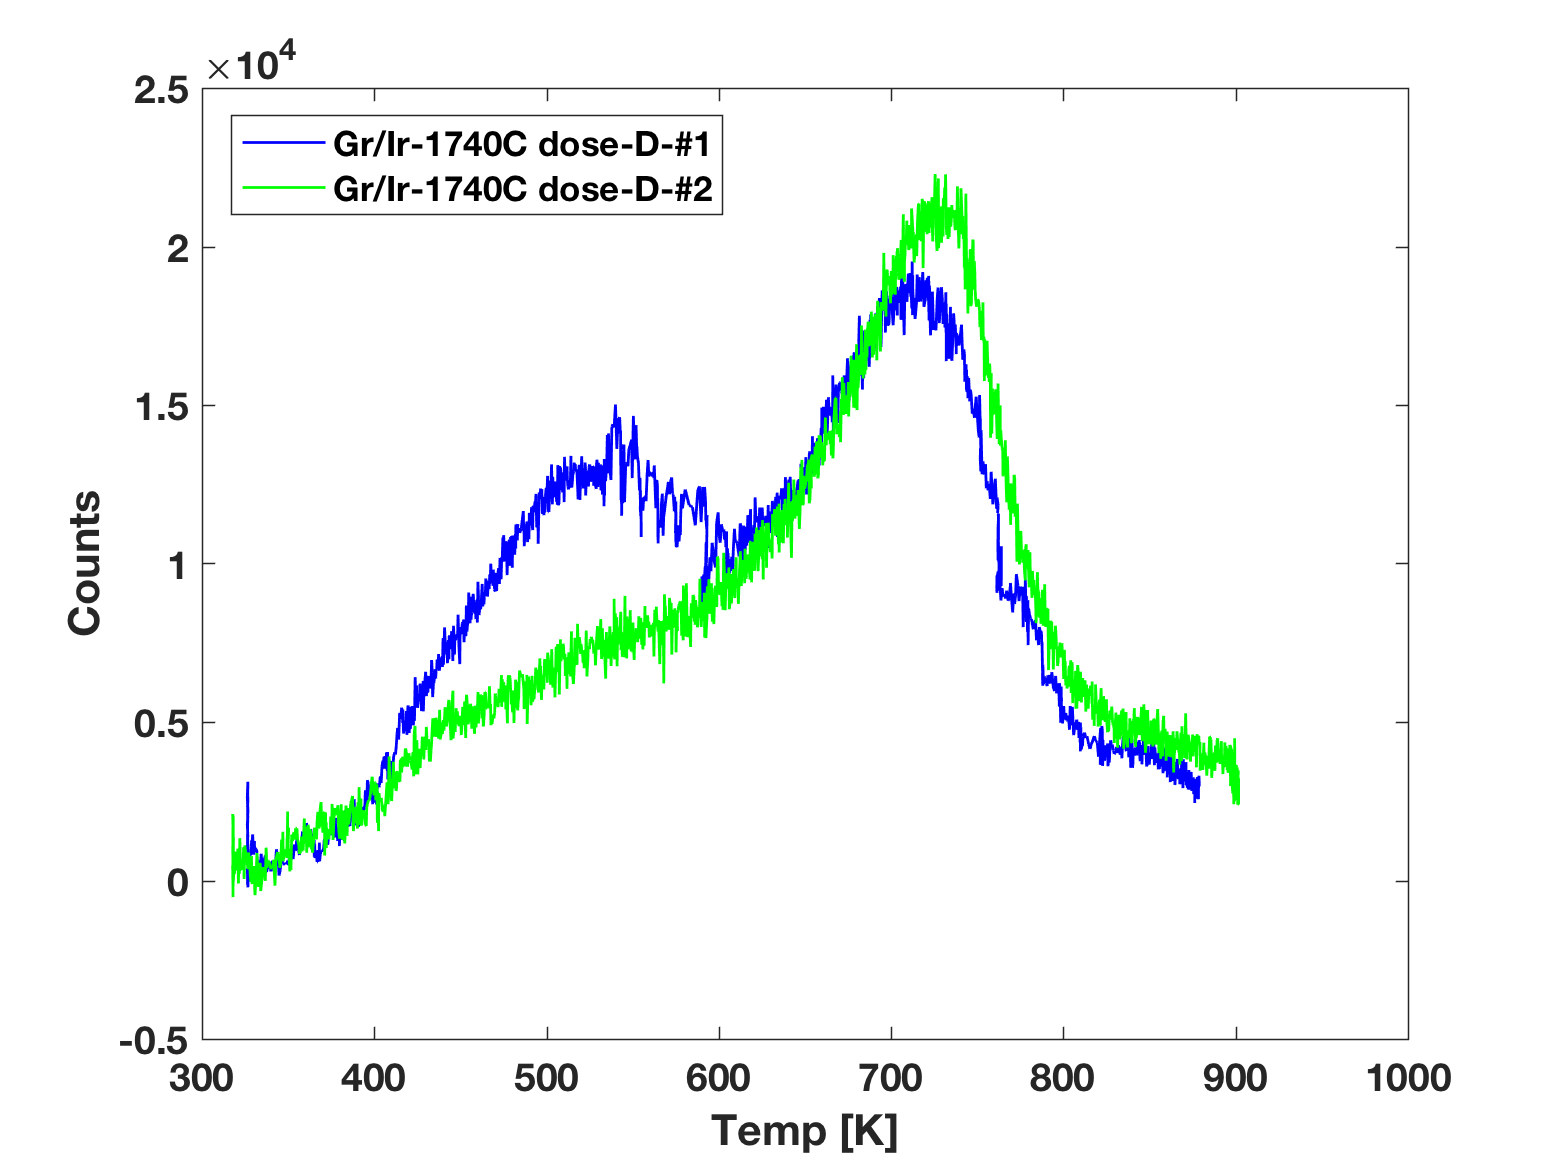
\includegraphics[width=\textwidth]{TPD/050516IrSorenDdose1hourtemp.png}
    \caption{TPD of Gr/Ir after 1 hour dose of atomic hydrogen with a doser temperature of 1740 \degree C.}
    \label{TPD:D}
  \end{subfigure}
  \caption{TPD measurements following doses of D$_2$ and hot atoms. (a) shows two graphs following from D$_2$ doses and (b) shows two graphs following from doses with hot atoms}
  \label{TPD:all}
\end{figure}

\section{Graphene bilayered sample}

As a further study of the adsorption of hydrogen on Gr/Ir, patches of graphene bilayers were grown on the sample by annealing in ethylene for a long period of time. The sample was investigated with several techniques, and the results are presented in the following sections.

\subsection{TPD of bilayered sample}
TPD measurements were conducted on the sample before and after the long anneal. The red graph in figure \ref{TPD:bilayer} is the results following a 60 min dose of D$_2$ at a chamber pressure of $1.04\cdot10^{-6}$mbar and with a doser temperature of 1740\degree C. The number of D$_2$ counts at the peak is roughly 13.000, which is a lot higher than the peaks in figure \ref{TPD:D2} with peak values around 8.000-9.000. This indicates that the surface was not saturated during the previous TPD measurements. Besides the higher peak value, the graph looks similar to the previous data, with a single peak around 700K.\\
The green graph corresponds to the sample after bilayers supposedly were grown. Bilayers were grown by exposing the sample to ethylene at a pressure of $1\cdot 10^{-6}$mbar for 60 min, while the sample was heated to 990\degree C. The sample was dosed with atomic hydrogen at a chamber pressure of $1.04\cdot 10^{-6}$mbar and with a doser temperature of 1740K as well as before. It is seen that the peak value this time is around 6.000, which means that the increased amount of bilayers reduce the amount of hydrogen on the surface by a significant amount. This suggests that hydrogen is not adsorbed on the bilayered graphene. This theory is supported by the STM pictures below.\\
It should be noted that only two datasets were gathered from this experiment. The peak intensity from the TPD measurements tends to vary slightly and hence the amount of bilayers grown on the sample might not be perfectly related to the drop in peak intensity.
\begin{figure}[H]
  \centering
  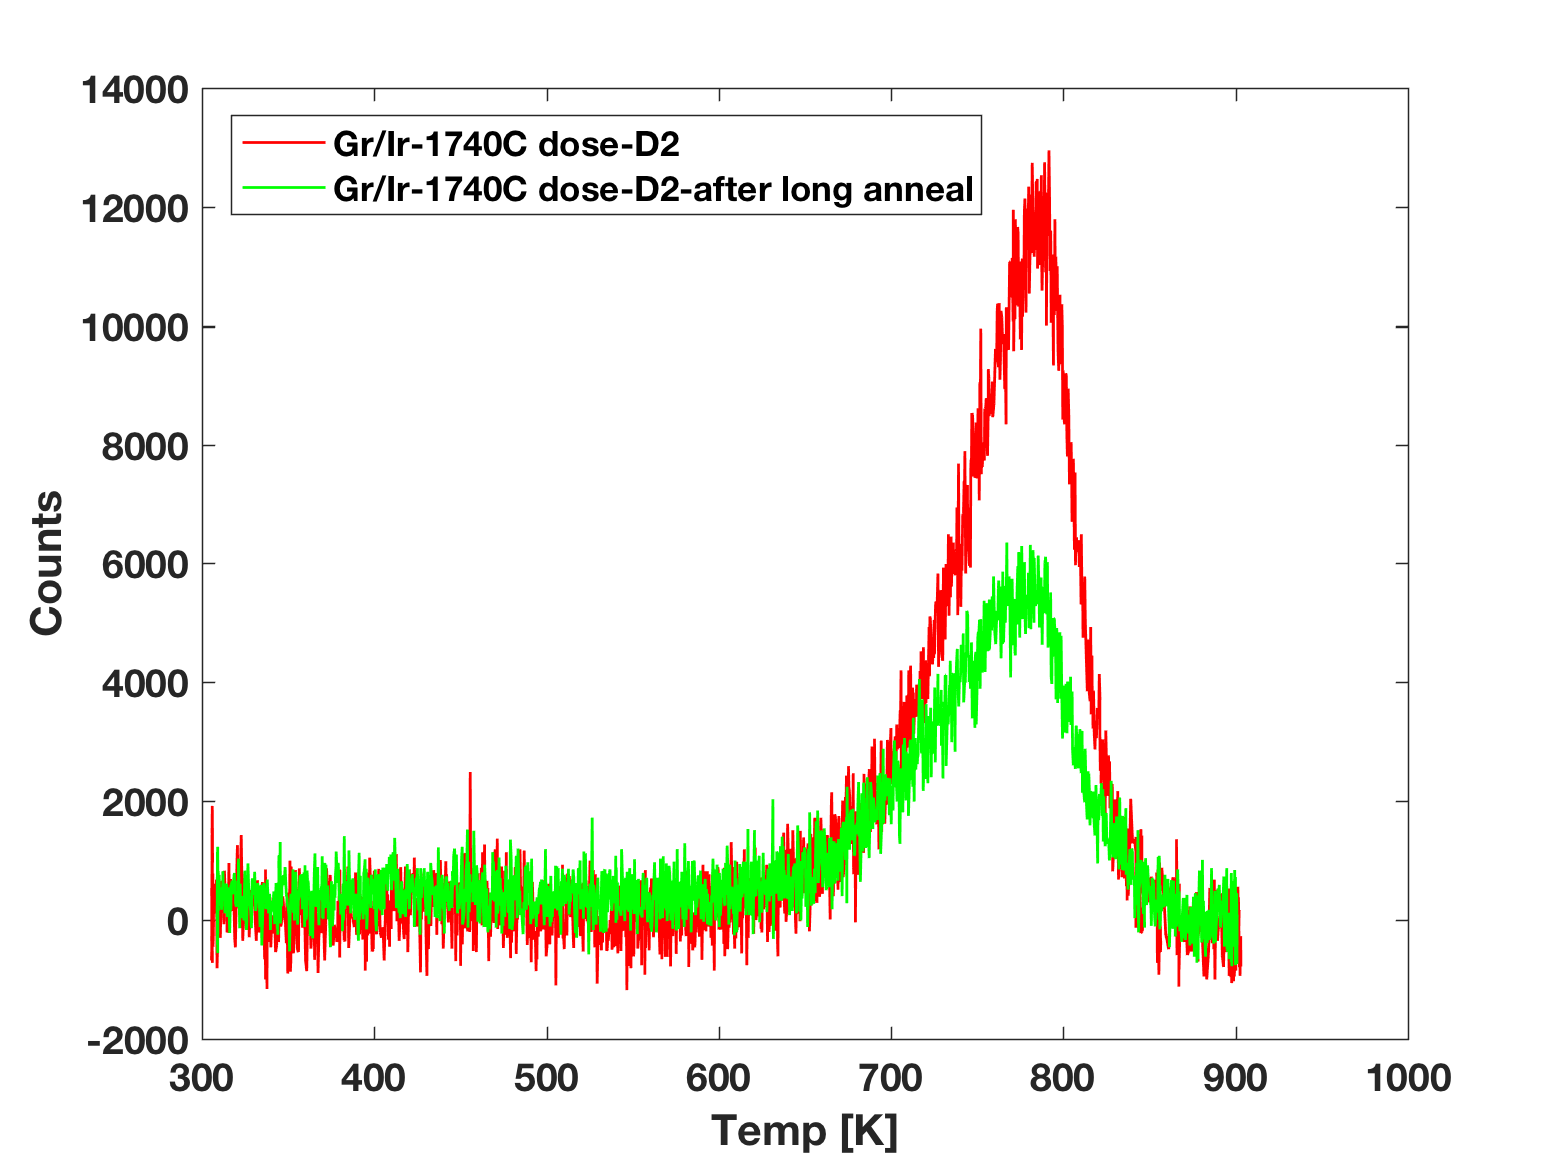
\includegraphics[width=0.6\textwidth]{TPD/GrIr1740CD2longannealtemp.png}
  \caption{TPD measurements after doses of D$_2$ at a pressure of $1.04\cdot10^{-6}$ and a doser T of 1740\degree C. The red graph is prior to a 60 min growth of bilayers where the 990\degree C hot sample was exposed to ethylene for 60 min at a pressure of $1\cdot10^{-6}$mbar}
  \label{TPD:bilayer}
\end{figure}

\subsection{STM images of bilayers}

In the following section STM images of bilayer patches are included. These images are made prior to the long anneal, and are therefore not directly related to the experiment mentioned in the preceding section. It was not possible to make images of the sample after the long anneal in ethylene, since the STM was broken. Bilayers were however present on the surface prior to the long anneal, and the following images show some of the key points about these.\\
The images in figure \ref{D2:} are made after the 12 hour dose of hydrogen at a chamber pressure of $1\cdot 10^{-5}$mbar with the ion gauge turned on. Hence the surface is fully hydrogenated which is somehow different to see due to the large images. On figure \ref{D2:bilayer1}, the three-point-star-structures characteristic for the hydrogenated surface are however seen, which is pointed out with the blue arrows. Bilayer patches are seen on the top half of the figure, and none of the structures characteristic for the fully hydrogenated surface are seen. A new superstructure is however seen with the individual flower-like structures, with a center circle surrounded by six other circles, construct a bigger pattern.\\
On figure \ref{D2:bilayer2} a linescan was made across the edge of the graphene monolayer-bilayer edge. The corresponding line profile is shown in figure \ref{linescanbilayer1}, and from this the height difference is measured to 2.97 $\pm$ 0.5Å. The bilayer edge is therefore significantly higher than the Iridium step edge, and much closer to the layer height of HOPG which is 0.35nm.\cite{PhysRevB.79.195429}\\
In order to investigate the bilayer superstructure further, a zoom in of figure \ref{D2:bilayer2} was made as seen in figure \ref{D2:bilayer3}. The graphene sheet is seen due to the atomic resolution, and it is obvious that no hydrogen is adsorbed to the surface. This is consistent with the data from the TPD measurements. Furthermore it is seen that the consistency in the superstructure is absent. Some areas of the bilayer has a cluster of three circles forming a triangle that points either up or down. These are highlighted in the left side of the picture. Other areas seem to have the flower-like structure mentioned earlier, but with an overlapping hexagon. An attempt to determine the periodicity of the superstructure was done by doing a linescan between two identical parts of the pattern. As seen on figure \ref{D2:bilayer3} the linescan was drawn between two down facing triangles, and the distance between these were measured from the bottom corner. The line profile is shown in figure \ref{linescanbilayer2} and the length between the points is measured to 45.78 $\pm$ 1Å.

\begin{figure}[H]
\makebox[\textwidth][c]{
  \begin{subfigure}[b]{0.3\paperwidth}
    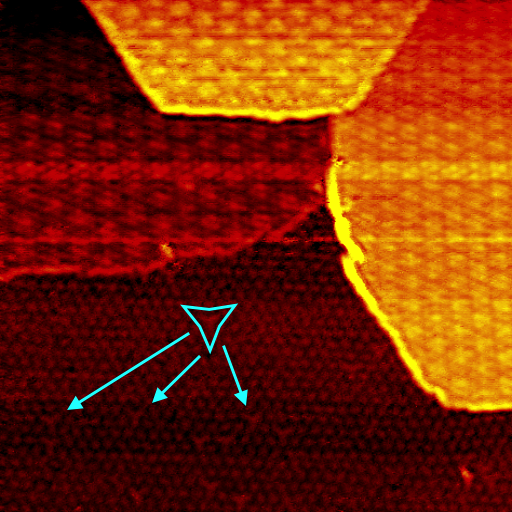
\includegraphics[height=\textwidth]{STMdata/FFT/2016-04-13_001_49.png}
    \caption{940x940 Å - 0.850 nA 75.7 mV}
    \label{D2:bilayer1}
  \end{subfigure}
  \begin{subfigure}[b]{0.3\paperwidth}
    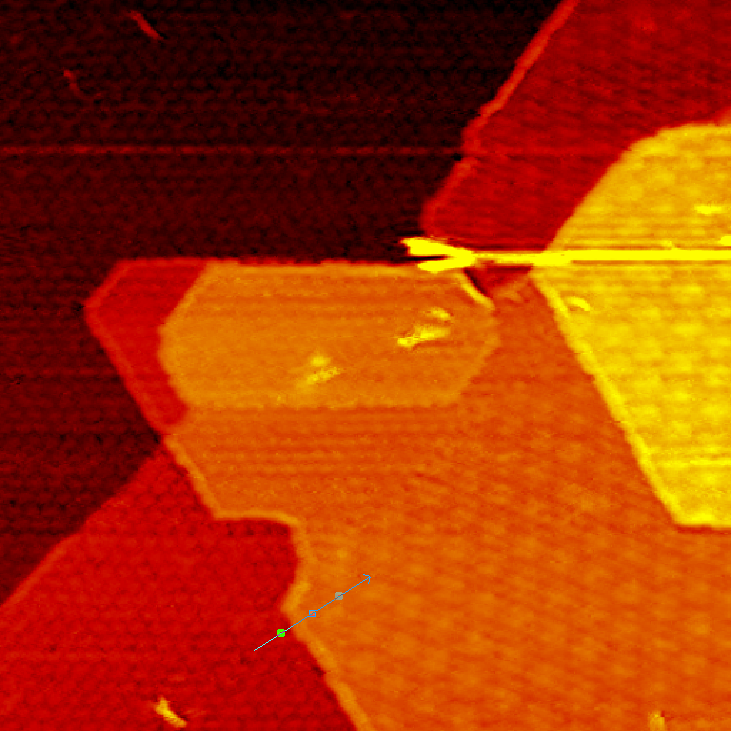
\includegraphics[height=\textwidth]{STMdata/FFT/2016-04-13_001_50.png}
    \caption{928x928Å - 0.800 nA 75.7 mV}
    \label{D2:bilayer2}
  \end{subfigure}
  \begin{subfigure}[b]{0.3\paperwidth}
    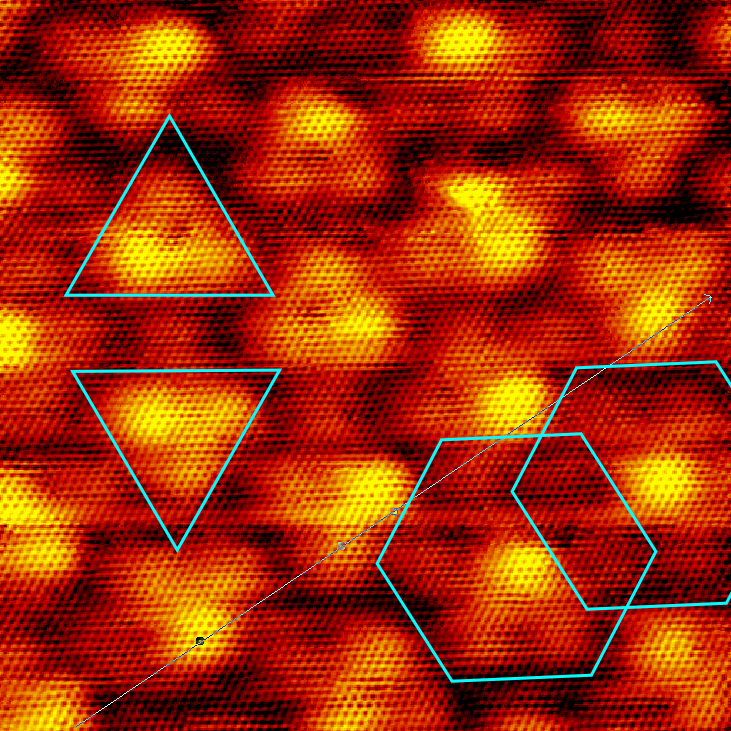
\includegraphics[height=\textwidth]{STMdata/FFT/2016-04-13_001_55.png}
    \caption{196x196 Å - 0.820 nA, 75.7 mV}
    \label{D2:bilayer3}
  \end{subfigure}
}
\\
\makebox[\textwidth][c]{
\begin{subfigure}[b]{0.35\paperwidth}
  \includegraphics[width=\textwidth]{STMdata/FFT/linescanbilayer1}
  \caption{Line profile belonging to the linescan in (b)}
  \label{linescanbilayer1}
\end{subfigure}
\begin{subfigure}[b]{0.35\paperwidth}
  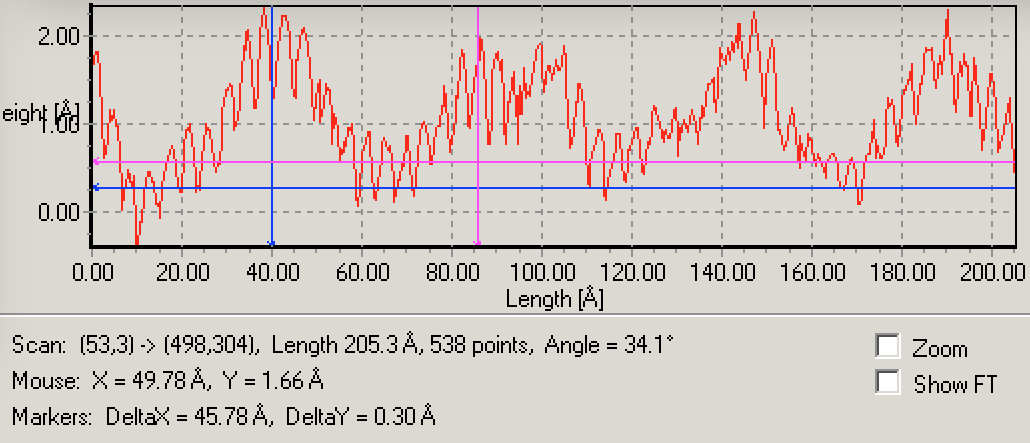
\includegraphics[width=\textwidth]{STMdata/FFT/linescanbilayer2}
  \caption{Line profile belonging to the linescan in (c)}
  \label{linescanbilayer2}
\end{subfigure}
}
\caption{Patches of bilayered graphene on Ir after a hydrogen dose at $1\cdot 10^{-5}$mbar for 12h.}
\label{D2:bilayer}
\end{figure}


\subsection{LEED of bilayered sample}
LEED was performed on the sample after an ethylene anneal with a chamber pressure of $7\cdot 10^{-7}$mbar. The figures in \ref{LEED} show pictures of the fluorescent screen within the UHV chamber from which the LEED was performed. The image on figure \ref{LEED1} shows the fluorescent screen after the untreated sample was exposed to an electron beam with an energy of 145eV. The spots marked out with the marked arrows show the diffraction pattern from the underlying Ir(111) surface, as well as the graphene sheet on top of the surface.\cite{1367-2630-10-4-043033}\\
The sample was then flashed to a low temperature in order to maintain any bilayers, and the sample was once again exposed to an electron beam of energy 145eV. The top and bottom right corner of the hexagonal pattern is enlarged in figure \ref{LEED2}. From this figure it is clear that some extra spots appear around the Ir and C spots pointed out in the previous figure. These spots arise from the moiré pattern of the graphene on Ir(111) surface. The reason why these spots were absent in the previous figure might be caused by a high amount of contaminants on the surface. These ruin the periodicity of the surface, and hence also the electron scattering, which then becomes smeared out. After annealing to a low temperature these contaminants should be gone, leaving the surface clean with small patches of bilayered graphene. The patches of bilayered graphene should however also cause a different scattering due to the changed periodicity as seen in figure \ref{D2:bilayer3}. If figure \ref{LEED2} and \ref{LEED3} is compared it does look like the spot belonging to the carbon atoms and the surrounding moiré spots in figure \ref{LEED2} are less distinct. These results might therefore indicate that bilayers are present on the surface in figure \ref{LEED2} and to a lesser extent in figure \ref{LEED3}. Since the picture in figure \ref{LEED3} is taken prior to an 1090\degree C anneal, it is reasonable to conclude that the bilayer patches desorb from the surface when annealing to this temperature.[Reference til desorption af bilayers?]

\begin{figure}[H]
\makebox[\textwidth][c]{
  \begin{subfigure}[b]{0.3\paperwidth}
    \includegraphics[height=\textwidth]{LEED/No" "flash/145eV.JPG}
    \caption{LEED without flashing. 145eV.}
    \label{LEED1}
  \end{subfigure}
  \begin{subfigure}[b]{0.3\paperwidth}
    \includegraphics[height=\textwidth]{LEED/Low" "T" "flash/145eV.JPG}
    \caption{LEED after low T flash. 145eV}
    \label{LEED2}
  \end{subfigure}
  \begin{subfigure}[b]{0.3\paperwidth}
    \includegraphics[height=\textwidth]{LEED/post" "1090" "flash/145eV.JPG}
    \caption{LEED after 1090\degree C flash. 145eV}
    \label{LEED3}
  \end{subfigure}
}
\caption{LEED pictures from the Gr/Ir sample with bilayers. [Reference til Antonija/Hoffmanlab]}
\label{LEED}
\end{figure}
